\documentclass{revtex4}
\usepackage{graphicx}
\usepackage{amsmath}
\usepackage{amssymb}
\usepackage{braket}
\usepackage{mathtools}
\usepackage{textcomp}
\usepackage{algorithm}
\usepackage{booktabs}
\usepackage{float}
\usepackage{caption}
\usepackage{color}
\linespread{2}
\begin{document}

\title{Hartree-Fock Stability Theory and its Relation to Correlation Theories}
\author{Evan Curtin}
\maketitle


\section{Background Information and Accomplishments}

   
   \subsection{Hartree-Fock Stability}
    Hartree-Fock (HF) Theory has been the foundation for \emph{ab initio} electronic structure 
    theory 
    throughout its history. An often overlooked aspect of the theory is that there are many 
    solutions to the HF equations for a given system, but being a 
    solution to the Hartree-Fock equation ensures only that the solution is stationary with respect 
    to the 
    determined orbitals. If the solution is indeed a minimum, it is called "stable", while if there 
    is any displacement in the electronic structure which reduces the energy, the solution is 
    "unstable". A method for determining the stability of a Hartree-Fock solution was 
    proposed by Thouless in 1960\cite{Thouless1960}. The condition was rederived into the 
    expression familiar to quantum chemists by Čížek and Paldus in 1967\cite{Cizek1967}. 
    Furthermore, the stability equations factorize depending on the symmetry of the Hartree-Fock 
    eigenfunctions. To this end, Seeger and Pople outlined a hierarchical approach to 
    systematically evaluate the stability of HF states in the restricted, unrestricted and 
    generalized Hartree-Fock procedures\cite{Seeger1977}. Recently, the method has been used to aid 
    the in search for the lowest energy Unrestricted Hartree-Fock (UHF) solutions in molecules, as 
    well as the General Hartree-Fock (GHF) solutions in geometrically frustrated hydrogen rings 
    which cannot conform even to the UHF scheme \cite{Pulay2016}\cite{Goings2015}.
    
    The usual method of determining stability of a Hartree-Fock solution is to look for a negative
    eigenvalue the Electronic Hessian, 
    \begin{equation}
     \bf{H}=
     \begin{bmatrix}
     \bf{A} &\bf{B} \\
     \bf{B}^* & \bf{A}^* \\
     \end{bmatrix},
    \end{equation} 
    where the matrices $\mathbf{A}$ and $\mathbf{B}$ have dimension $N_{occupied} \times 
    N_{virtual}$ with elements given by
    \begin{align}
     A_{i \rightarrow a, j \rightarrow b} &= (\epsilon_a-\epsilon_i)\delta_{ij}\delta_{ab} 
     + \left< aj||ib \right>, \\
     B_{i \rightarrow a, j \rightarrow b} &= \left< ab||ij \right>. 
    \end{align}    
    If $\bf{H}$ has a negative eigenvalue, this indicates an 
    instability. For a paramagnetic HF solution, the equations 
    factorize into the matrices known to 
    chemists as the singlet and triplet instability matrices \cite{Dunning1967}\cite{Seeger1977},
    
     \begin{subequations}
     	\begin{align}
     	{}^{1}{A'}_{i\rightarrow a, j\rightarrow b} &= (\epsilon_a-\epsilon_i)\delta_{ij}\delta_{ab} 
     	+ 2\braket{aj|ib}-\braket{aj|bi}\\
     	{}^{3}{A'}_{i\rightarrow a, j\rightarrow b} &= (\epsilon_a-\epsilon_i)\delta_{ij}\delta_{ab} 
     	- \braket{aj|bi}\\
     	{}^{1}{B'}_{i\rightarrow a, j\rightarrow b} &= 2\braket{ab|ij}-\braket{ab|ji}\\
     	{}^{3}{B'}_{i\rightarrow a, j\rightarrow b} &= -\braket{ab|ji}
     	\end{align}
     \end{subequations}
     where the $1,3$ denote singlet and triplet instabilities, respectively. The lowest eigenvalue 
     of both of 
     these matrices will reveal the stability of the RHF solution. If they are both positive, the 
     solution is stable with respect to symmetry breaking, while negative eigenvalues in either 
     indicate instability with respect to either triplet or singlet perturbations (or both). An 
     eigenvalue of 0 does not indicate instability, and this case is discussed 
     in detail by Cui et al \cite{Cui2013}.
    
    \subsection{Hartee-Fock Stability of the Homogeneous Electron Gas}
    
    The Homogeneous Electron Gas (HEG) model of metallic systems is a convenient starting point 
    for 
    this study. The Energies of various phases thereof have been computed to great accuracy
    \cite{Ceperley1980}, while plane wave solutions to the Hartree-Fock equations can be 
    demonstrated analytically \cite{Phillips2012}. Furthermore, within the Hartree-Fock 
    approximation, it has been known for half a century that broken symmetry solutions are always 
    lower in energy compared to their paramagnetic counterparts \cite{Overhauser1962}. More 
    recently, phase diagrams have been determined for the 
    HEG in 2 and 3 dimensions\cite{Delyon2008}\cite{Bernu2011}\cite{Baguet2013}. In all cases the 
    phase diagrams are made by computing the energies of the polarized and unpolarized states, and 
    comparing them. This approach necessitates that the form of the solutions is known ahead of 
    time. 
    
    The present work focuses on directly calculating the Hartree-Fock stability of 
    the 
    paramagnetic homogeneous electron gas as a function of electron density. In this way it is 
    possible to map out where the symmetry broken Hartree-Fock reference is needed. 
    	
  \subsection{Method}

	Starting with the Jellium Hamiltonian in atomic units, 
	\begin{equation}\label{hamiltonian}
		\hat{H} = \sum_i \frac{\hat{p}_i^2}{2}  + \frac{1}{2} \sum_{i < j} \frac{1}{|\vec{r}_i - 
		\vec{r}_j|},
	\end{equation}
	one solution to the Hartree-Fock equations in $D$ dimensions are plane waves of the form	
	\begin{equation}\label{planewave}
		\phi_{\vec{k}} =
		   \frac{1} { \sqrt{L ^ D} } e ^ {i \vec{k} \dot \vec{x}},
	\end{equation}
	where $L$ is the length of one side of the direct lattice with cubic symmetry. Using this as the 
	basis for the rest of the analysis, the two electron repulsion integrals are analytic and 
	well-behaved in two and three dimensions \cite{Delyon2008}\cite{Guiliani2005}
  \begin{align}
   	\braket{\vec{k}, \vec{k}' | \vec{k}'', \vec{k}'''} 
  	  \stackrel{ \text{2D, 3D} }{=}&
   	\begin{cases} 
   	\frac{\pi} {\Omega} \frac{ 2^{D-1} } { | \vec{k} - \vec{k}'' | ^ {D-1} } 
   	& \vec{k}''' = \vec{k} + \vec{k}' - \vec{k}'' + n\vec{G} \textbf{ and } | \vec{k} - 
   	\vec{k}''| \neq 0 \\
   	0 
   	& \text{else}
   	\end{cases}
  \end{align}
  where $\Omega$ is the direct lattice volume and $n\vec{G}$ is any integer times a reciprocal 
  lattice vector of the 
  system. The orbital energies are
  \begin{equation}\label{eq:hf_orb_energy}
  \epsilon_{\vec{k},\sigma}=
  \frac{\hbar^2\vec{k}^2}{2m} - \sum\limits_{\vec{k}}^{|\vec{k}|< 
  k_f}n_{\vec{k}\sigma}\braket{\vec{k}, \vec{k}' |\vec{k}', \vec{k}},
  \end{equation}
  where $n_{\vec{k}\sigma}$ is the occupation number of the state with momentum $\vec{k}$ and 
  spin $\sigma$ \cite{Guiliani2005}. 
    
 \subsection{Results}   
      Using the equations for energies and two electron integrals, the stability analysis was 
      performed on the paramagnetic HEG model as a function of electron density (or equivalently, 
      $r_s$). The naive approach of explicitly constructing and diagonalizing the orbital hessian 
      is intractable both in terms of memory and calculation time requirements. Since the 
      instability condition is that the any eigenvalue is negative, it suffices to calculate the 
      sign of only the lowest eigenvalue. This is a task well suited for an iterative subspace 
      solver. To this end a parallel version of the Jacobi-Davidson algorithm 
      was implemented by representing the matrix as a matrix-vector product (made possible by the 
      SLEPc library\cite{Hernandez2005}). This allowed for two necessary optimizations. First, the 
      algorithmic change from full diagonalization to a subspace algorithm reduces the memory 
      requirements from $O(N^2)$ to $O(N)$ and the computational scaling from $O(N^3)$ to $O(N^2)$. 
      Secondly, the parallelization of the algorithm allows the program to be run on the Blue 
      Waters supercomputer with about 80\% strong parallel scaling efficiency. 
     \begin{figure}[H]
       \centering
       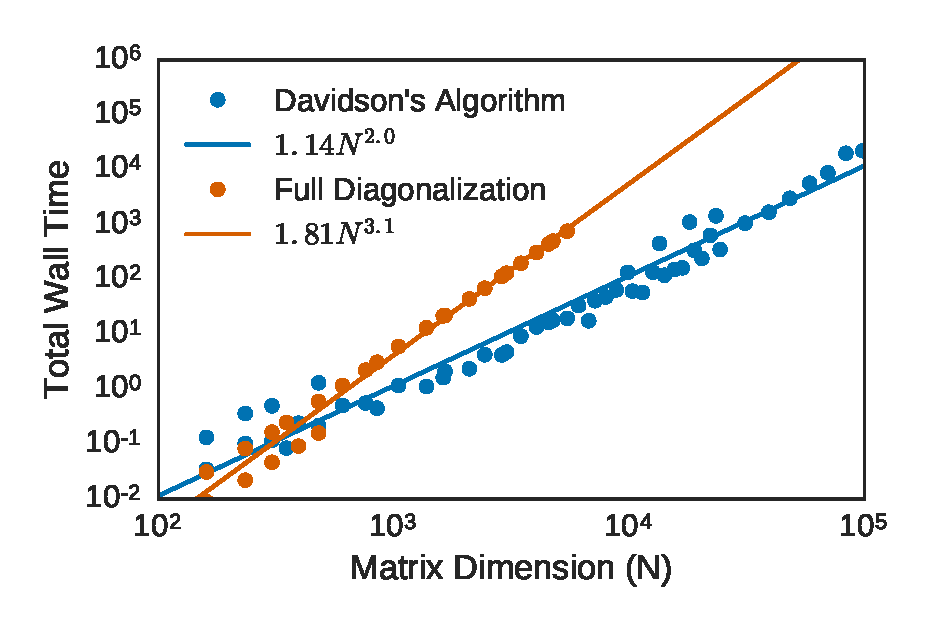
\includegraphics[width=0.5\textwidth]{../figures/dav_vs_exact_scaling.eps}
       \caption{The asymptotic scaling of both algorithms behaves as expected.}
     \end{figure}  
     \begin{figure}[H]
     \centering
      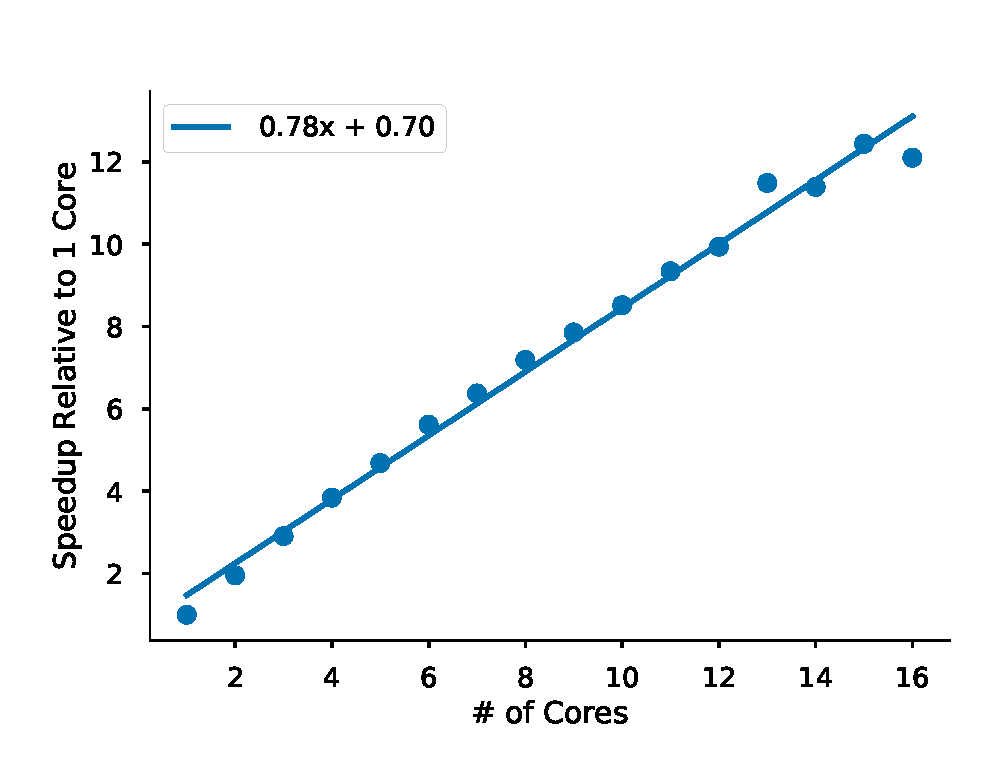
\includegraphics[width=0.5\textwidth]{../figures/parallel-scaling.eps}
      \caption{The speedup of the entire calculation as the number of computer cores is 
      sufficiently linear.}
     \end{figure}     
     These optimizations allow the calculation to be performed with enough grid points to         
      \begin{figure}[H]
      \centering
        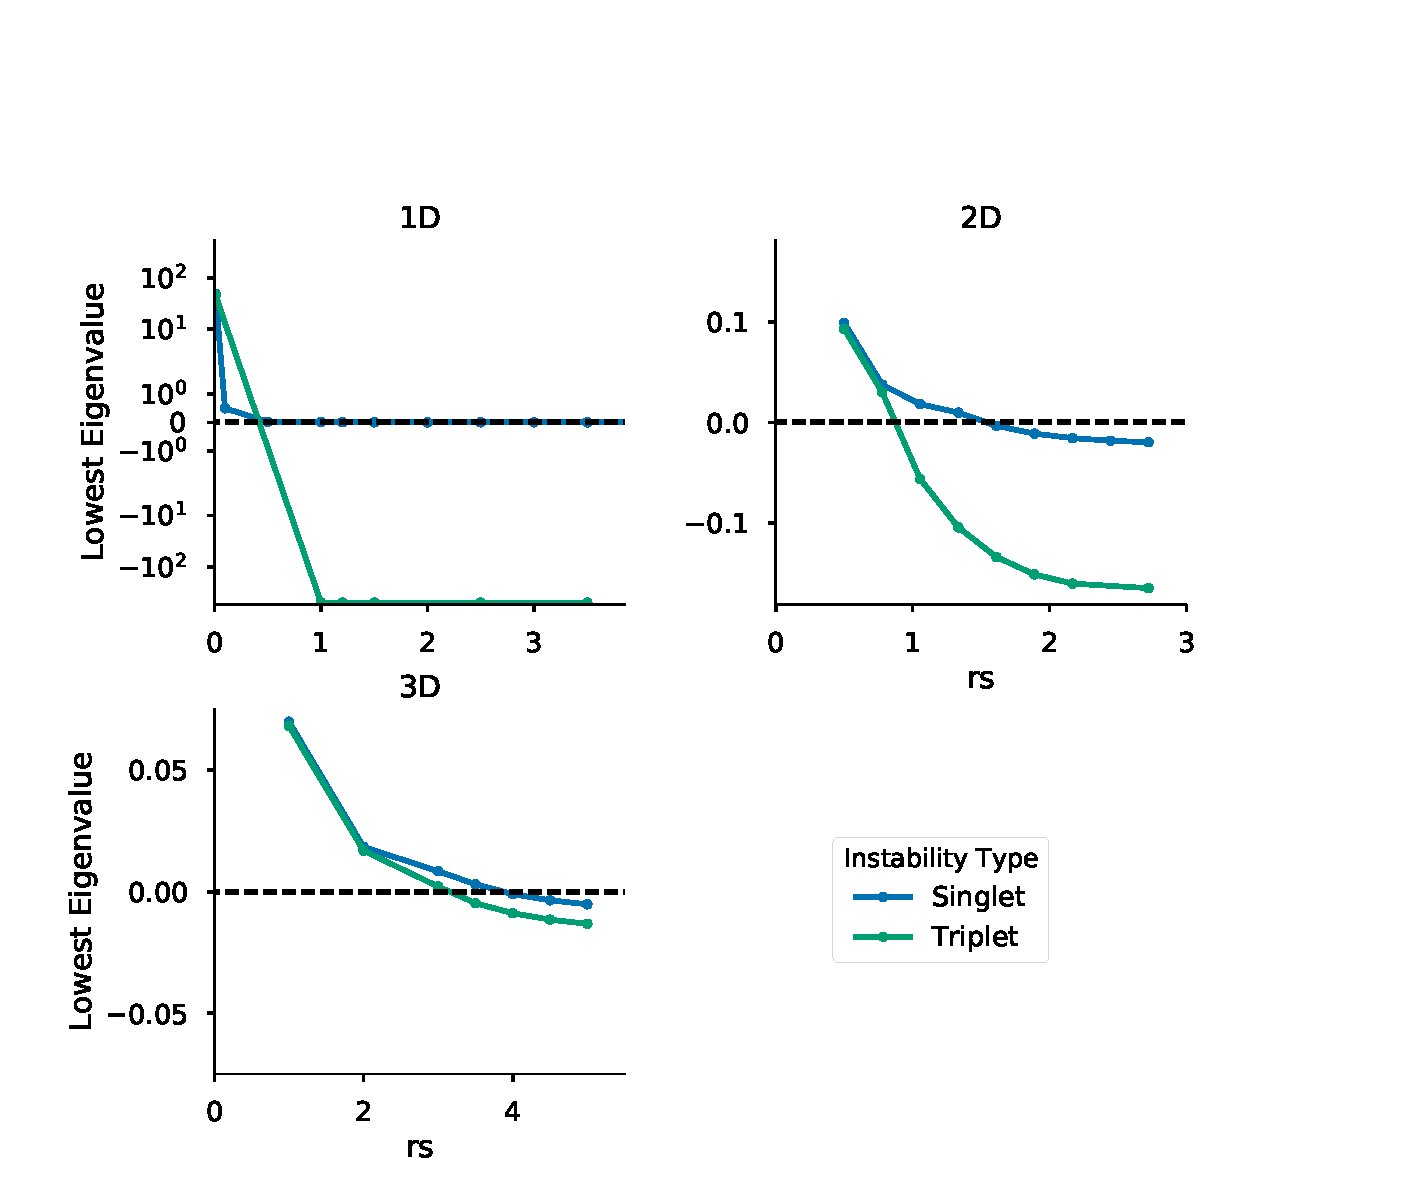
\includegraphics[width=0.75\textwidth]{../figures/stability.pdf}
        \caption{The Lowest eigenvalues of the triplet and singlet instability matrices in 1, 2 and
        3 dimensions.}
      \end{figure}   
        
    In each case, there is a clear density at which the triplet instability appears, and persists 
    beyond. Tracking this quantity as a function of number of grid points in the calculation 
    reveals that this "transition $r_s$" occurs at $r_s = 1$ in 2D and $r_s = 3$ in 3D. These 
    results are consistent with those seen by other methods. 
    \cite{Baguet2014}\cite{Bernu2011}

    \begin{figure}[H]
    \centering
      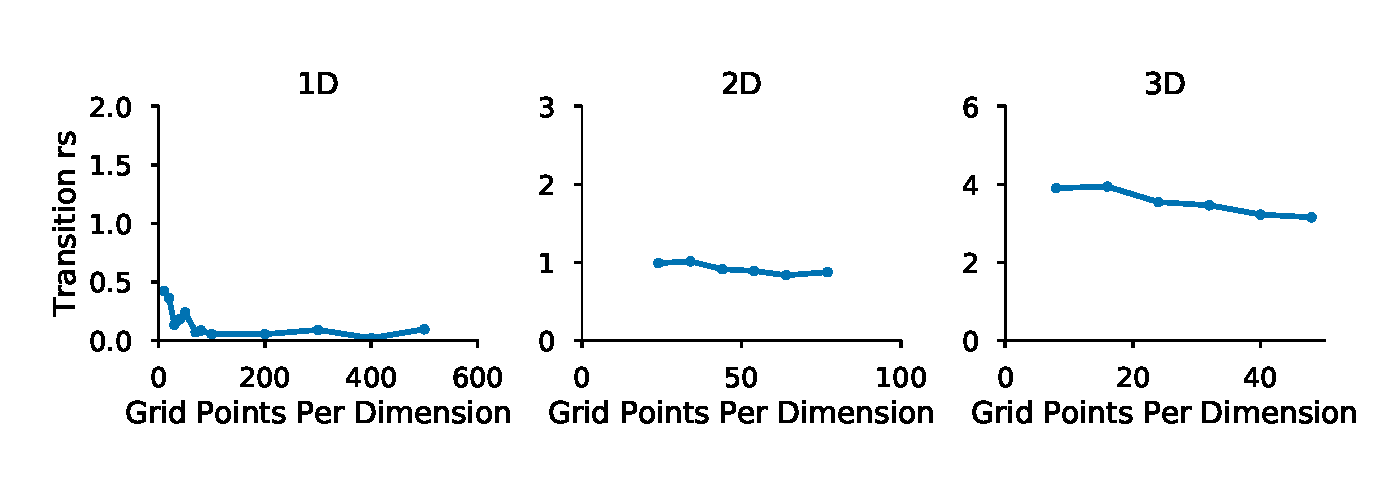
\includegraphics[width=0.75\textwidth]{../figures/triplet_onset.eps}
      \caption{The Lowest eigenvalues of the triplet and singlet instability matrices in 1, 2 and
      3 dimensions.}
    \end{figure}
    
    
\newpage
\section{Goals and Relevance of Proposed Research}
    The goal of electronic structure theory is to solve the electronic Schr{\"o}dinger equation
    for a molecule or solid state system. The prevailing approach in \emph{ab initio} quantum 
    chemistry is to first compute a self-consistent single-determinant Hartree-Fock (HF) solution 
    which will serve as a reference for many-body perturbative (MP) or coupled-cluster (CC) 
    approaches.  
    Implicit in these methods is the assumption that the reference wave function will be 
    sufficiently close to the exact solution of the Schr{\"o}dinger equation to converge to the 
    correct 
    answer in a computationally feasible manner. Both the MP and CC approaches have the attractive 
    quality that they are systematically improvable, i.e. more computational power can be used on a 
    problem to increase the accuracy of the resulting solution. These so-called post-Hartree-Fock 
    methods are able to recover more of the total electronic energy by accounting for the 
    \emph{correlation energy} in the system. Traditionally, the correlation energy is defined by 
    the difference between the exact energy and the Hartree-Fock energy \cite{Shavitt2009}
    \begin{equation}\label{correlation_energy}
      E_{corr} = E_{exact} -  E_{HF}
    \end{equation}
    In many cases the correlation energy is relatively small and the Hartree-Fock reference 
    captures a significant portion of the exact total energy. In such cases, the prevailing 
    approach is usually successful and has only implementation issues for larger systems. On the 
    other hand there are systems which are not well treated by this approach, which are often 
    called "strongly correlated". Examples of such systems are those with degenerate or 
    near-degenerate HOMO-LUMO gaps, metallic solids or molecules close to breaking bonds. 
    Oftentimes for such systems the traditional Hartree-Fock solutions are not even qualitatively 
    correct, implying inadequacies in either the single-reference or mean-field approach. 
      
      It is often neglected, however, that the usual way for computing a Hartree-Fock solution in 
      practice
    is to use a restricted form of the single determinantal wavefunction. In the Restricted 
    Hartree-Fock (RHF), the wave function is restricted to be an eigenfunction of the $\hat{S^2}$ 
    and $\hat{S_z}$ 
    operators, while in the Unrestricted variant (UHF), the wave function need only be an 
    eigenfunction 
    of the $\hat{S_z}$. There is yet another lesser-known variation of the theory, known as General 
    Hartree-Fock (GHF), which assumes no spin-symmetries in the wave function. This allows for 
    greater
    variational flexibility at the cost of "broken symmetry". Together these three levels of 
    Hartree-Fock theory form a heirarchy of increasing parameter space within which to minimize the 
    total energy. Thus the term "Hartree-Fock Energy" is inherently ambigious; this fact calling 
    into question commonly held ideas about correlation and Hartree-Fock theory. Take for example 
    the dissociation curve of H$_2$ in the RHF and UHF approximations, compared with the exact 
    solution obtained by full configuration-interaction in the complete basis set limit. 
    
    \textcolor{red}{H2 curve pic}
    
    The correlation energy for the RHF reference case is dramatically larger than that for the UHF 
    reference. In other words, \emph{the correlation energy is, by definition, inherently coupled 
    to the 
    Hartree-Fock reference}. The given example is well understood, but it brings to mind a more 
    general idea that there may be more cases where apparently large correlation energies are due 
    to simply 
    using and inadequate level of Hartree-Fock theory. Scuseria and coworkers have leveraged this 
    idea to create new coupled cluster theories while preserving the symmetry of the reference 
    \cite{Gomez2016}. While the exact wave function of will have the same symmetry as the exact 
    Hamiltonian, it is important to remember that the Hartree-Fock Hamiltonian is not exact, and we 
    may have something to gain by taking the variational principal at face value; lower energy is 
    always better. For certain observables this is not the case, but for energies alone we are free 
    to maintain this mindset. Therefore the overarching theme of the proposed work is that 
    \emph{many 
    examples of strong correlation may be illusory, and in order to find out we have to find lower 
    energy Hartree-Fock solutions, even at the cost of broken symmetry}.    

\section{References}
\bibliography{../prelim_references}

\end{document}